\documentclass[10pt,a4paper]{article}
\usepackage[margin=2.1cm]{geometry}
\usepackage[T1]{fontenc}
\usepackage{lmodern}
\usepackage{microtype}
\usepackage{amsmath,amssymb}
\usepackage{booktabs,tabularx,longtable,multirow,xltabular}
\usepackage{xcolor}
\usepackage{enumitem}
\usepackage{caption}
\usepackage{float}
\usepackage{tikz}
\usetikzlibrary{positioning,arrows.meta,fit,backgrounds}
\usepackage[colorlinks=true,linkcolor=blue!50!black,citecolor=blue!50!black,urlcolor=blue!50!black]{hyperref}

\setlist{nosep,leftmargin=1.4em}
\captionsetup{font=small,labelfont=bf}
\newcolumntype{Y}{>{\raggedright\arraybackslash}X}
\newcolumntype{P}[1]{>{\raggedright\arraybackslash}p{#1}}
\newcommand{\pz}{$\pi_{0}$}
\newcommand{\pzf}{$\pi_{0.5}$}
\newcommand{\pzs}{$\pi_{0.7}$}
\DeclareRobustCommand{\meas}{\textsuperscript{\textcolor{green!50!black}{m}}}
\DeclareRobustCommand{\est}{\textsuperscript{\textcolor{orange!80!black}{e}}}
\DeclareRobustCommand{\pend}{\textcolor{gray}{pending}}
\newcommand{\pos}{\textcolor{green!45!black}{\textbf{+}}}
\newcommand{\negr}{\textcolor{red!70!black}{\textbf{--}}}
\newcommand{\neu}{\textcolor{gray}{$\circ$}}

\title{\textbf{A steerable, memory-equipped robot stack around open VLAs}\\[2pt]
\large Literature, experiments and results, design choices, end-to-end pipeline, data quality, gaps,\\ claims to verify, and compute}
\author{Robot learning team}
\date{Status report, 24 October 2026 (simulation and offline results)}

\begin{document}
\maketitle

\begin{abstract}
\noindent
We are building a robot stack that a person can \emph{steer} (change the command mid-task, point at targets, state preferences), that \emph{remembers} over minutes, that \emph{plans} at a high level and executes short low-level horizons, and that \emph{improves continuously} from its own deployment data, on top of open vision-language-action (VLA) models, with OpenArm~2 bimanual arms as the target hardware.
This report collects the literature we drew on, every experiment run so far with its results (all in simulation or on public recordings), the design choices they led to, the resulting end-to-end architecture and data pipeline, an assessment of the data we used, the gaps, the claims that still need verification, and the compute required.
\textbf{Main supported findings.} (i) A frozen flow-matching VLA (G0.5) follows a changed instruction only 13--29\% of the time; a 2\,s pointing nudge raises this to 39--49\% ($p\le0.007$ in every test), and learned noise policies reach the same level without a target point. Tested under realistic conditions inside multi-step missions, however, pointing precision does not matter (a VLM's 15\,cm-off points work as well as perfect ones), and simply \emph{retracting the arm and re-issuing the command} beats every pointing or learned method (51/53 vs 26/53 changed steps completed, $p=4\times10^{-7}$). (ii) An external memory module raises success after the instruction disappears from 40\% to 86\% ($p=10^{-10}$); in realistic interrupt-and-resume missions, only a planner given the robot's own activity log resumes at the right step (23--27/40 vs 0--7/40 with the conversation or the current view, $p\le3\times10^{-5}$, two planners), and storing standing instructions as explicit rules cuts violations from 20/30 to 0/30 ($p=2\times10^{-6}$); 4B planners ignore such instructions when they are only in their context. For state the camera cannot see (how many repetitions are done), a counter built from the robot's own activity log lifts closed-loop success from 5.8\% to 20.8\% ($p=3\times10^{-4}$), matching a learned video memory. (iii) A small latent world model turns the frozen VLA into a goal-conditioned planner (77\% vs 2--7\%). (iv) Preference-guided fine-tuning (PrefPI) raises a carried object's height by 52\% at $\approx$90\% success, but retraining on its own rollouts drifts the policy and degrades success by round 8; mixing in original demonstrations removes the drift, and whether the preference still accumulates is being tested. A second round of model-based steering improvement regressed because the refit critic became overconfident. (v) Among world models evaluated on real household recordings, FLUX~3 Action predicts folding motion best (0.70$\times$ the error of holding still); RoboJEPA improves smoothly with scale and supports gradient planning 4$\times$ faster than CEM; but used realistically as a motion verifier inside missions, a world model adds nothing measurable (57 vs 56/80 changed steps completed; with diverse proposals no better than a random pick). Moved up to the level of commands, it works: a small model that imagines the \emph{end state} of each candidate command from the current view reads every picture goal in the missions (53/53, vs 11/54 for a zero-shot 4B planner) and raises end-to-end mission completion from 3/80 to 26/80 ($p=1.6\times10^{-6}$), using only the camera and the goal photograph. Training G0.5's own weights through a learned world model and critic, by contrast, collapsed the policy (0/200) or, tightly anchored, did nothing; steering through the noise is the safe form. (vi) In a three-step mission benchmark that needs memory, a change of mind and a picture-only goal, the fully wired system completes 5/24 missions end to end, against 0/24 without the planner ($p=0.06$) and 1/24 without memory or without steering; removing memory cuts step-1 completion from 17/24 to 6/24 ($p=0.001$). Short horizons show no significant mission-level effect at this size; the motion-level world model none either, the command-level one a large one (above). All mission-level numbers need more missions and a real robot.
\end{abstract}

\noindent\small Legend: \meas\ measured on our runs; \est\ estimate; \pos/\negr/\neu\ positive/negative/neutral finding. Statistical tests are paired exact McNemar tests on shared start states with task-macro bootstrap 95\% CIs unless stated. ``pts'' = percentage points.\normalsize

\tableofcontents
\newpage

%==================================================================
\section{Goals and scope}
\label{sec:goals}
The target system must support, on OpenArm~2 hardware and household tasks (towel and cloth folding, washer loading/unloading):
\begin{enumerate}
  \item \textbf{Steerability}: react within seconds to a changed command, a pointed target, or a correction.
  \item \textbf{Memory}: keep task state and user intent over 1--15 minutes, beyond a Markovian VLA.
  \item \textbf{Preferences}: adjust style (speed, height, care) from sparse human feedback.
  \item \textbf{High-level planning}: decompose a task into short subtasks with explicit targets.
  \item \textbf{Short low-level horizons}: the VLA only executes $\approx$1\,s chunks of a 2--10\,s subtask; a command-level world model imagines the outcome of candidate subtasks for the planner (picture goals).
  \item \textbf{Continuous improvement}: post-training and RL from deployment data without regressions.
\end{enumerate}
A hard constraint is \textbf{licensing}: the deployed stack must use commercially usable weights (G0.5, Awomo-0.5, FLUX~3 and RoboJEPA are research-only or restricted; see \S\ref{sec:choices}).
All results here come from simulation (LIBERO, RoboCasa365) or public real-robot recordings (DROID); no OpenArm data has been used yet.

%==================================================================
\section{Literature review}
\label{sec:lit}

\subsection{Vision-language-action policies}
\textbf{Flow-matching VLAs.} \pz~\cite{pi0} and \pzf~\cite{pi05} pair a pretrained VLM with a flow-matching action expert; \pzs~\cite{pi07} adds subtask instructions, generated subgoal images and episode metadata (speed, quality, mistakes) amplified by classifier-free guidance (CFG) at inference. G0.5~\cite{g05} (Galaxea) is a single transformer for reasoning and action tokens with a flow-matching variant that reaches 98.9\% on LIBERO; it is our main research policy (non-commercial licence). GR00T N1.7~\cite{gr00t} (NVIDIA, open model licence) uses a Cosmos-Reason2 backbone and a DiT action head; Enactic released an OpenArm~2 checkpoint. LingBot-VLA 2.0~\cite{lingbot2} (Robbyant, Apache-2.0 code) is a 6B model with a Qwen3-VL-4B backbone, a 55-dimensional cross-embodiment action space, 10 denoising steps and $\approx$130\,ms inference on an RTX~4090D. Awomo-0.5I~\cite{awomo} is a strong RoboCasa365 policy under a non-commercial licence, used as a reference.
\textbf{Continual learning.} Pretrained VLAs are reported to be surprisingly resistant to forgetting~\cite{vla_forget}, which supports periodic fine-tuning in a flywheel.

\subsection{World models and world-action models}
Latent (JEPA-style) world models predict future encoder features instead of pixels: V-JEPA~2.1 features underlie RoboJEPA~\cite{robojepa} (22M--8B predictors trained on robot video, with CEM planning in latent space). LaWAM~\cite{lawam} pairs a latent world model (DINOv3 features) with a latent-action model for policy learning; FLARE~\cite{flare} aligns policies with future latents. Generative \emph{world-action} models jointly denoise future video and actions: Cosmos~3~\cite{cosmos3} (NVIDIA, OpenMDW licence; Edge and Nano sizes, DROID policy variants) and FLUX~3 Action~\cite{flux3a} (Black Forest Labs, 7B, FLUX Kommunity licence; video tokens are sampled but not decoded). OpenWAM~\cite{openwam} studies world-action pretraining systematically.
\textbf{Learning through learned dynamics.} Dreamer-style agents~\cite{dreamerv3} and TD-MPC2~\cite{tdmpc2} learn policies or plan inside learned models; SHAC~\cite{shac} uses short-horizon analytic gradients with a critic in a differentiable simulator. SuperMimic~\cite{supermimic} fits one differentiable world model to simulator transitions and trains a humanoid tracker by backpropagation through 32-step imagined rollouts plus a critic, surpassing a 128-GPU PPO baseline in 3 GPU-hours; it is the template for our model-based steering experiments.

\subsection{Steering frozen generative policies}
CFG~\cite{cfg} amplifies a conditional-to-unconditional density ratio; CFGRL~\cite{cfgrl} interprets it as a policy-improvement operator. Flow Reversal Steering (FRS)~\cite{frs} integrates a frozen flow policy backward from a coarse human/VLM reference action to a noise and forward again, yielding an in-distribution refinement; its extension trains a noise policy on successful steered noises (``DSBC'' in this report). DSRL~\cite{dsrl} and FlowDAgger~\cite{flowdagger} steer frozen diffusion/flow policies through the input noise; VLS~\cite{vls} uses VLM-derived rewards at inference; Imagining Recovery~\cite{imagrecovery} realigns VLAs with counterfactual futures. A user-supplied description of ``Cue the Flow'' (a spatial cue encoder with scale-and-shift adapters on a frozen \pzf) could not be located as a paper; we treat it as related to the noise- and cue-adapter family.

\subsection{Preferences and RL fine-tuning}
PrefPI~\cite{prefpi} conditions a policy on a ``[cfg]'' preference token trained on the top 40\% of its own rollouts and applies CFG ($w=5$) at inference, iterating to reach behaviours outside the initial policy's support (on \pzf\ in LIBERO: 25--38\% faster, +65\% carry height; on hardware: 10.7$\rightarrow$19.8\,cm from 150 labels). Baselines include Diffusion-DPO~\cite{diffdpo}, FDPP~\cite{fdpp} (reward model + DPPO~\cite{dppo}) and FlowPRO~\cite{flowpro}. \pzs's metadata conditioning~\cite{pi07} is the same mechanism with quality labels instead of preferences.

\subsection{Memory and high-level planning}
LIBERO-Mem~\cite{liberomem} and MIKASA-Robo-VLA~\cite{mikasa} show that Markovian VLAs fail tasks needing history; 3D-Mem~\cite{3dmem} selects event snapshots for embodied QA. High-level embodied VLMs such as RoboBrain~2.0/2.5~\cite{robobrain} and general VLMs such as Qwen3-VL~\cite{qwen3vl} can decompose instructions and point at targets; \pzs\ conditions its low level on such subtasks~\cite{pi07}.

\subsection{Benchmarks and data}
LIBERO~\cite{libero} (with robustness variants such as LIBERO-PRO~\cite{liberopro}), RoboCasa365~\cite{robocasa365} (365 kitchen tasks, atomic and composite, seen and unseen) and DROID~\cite{droid} (real Franka teleoperation) are our evaluation and data sources. A recent bimanual household study scaled from 1,500 hours of demonstrations to on-policy corrections~\cite{agibot}, the closest public analogue of our target data regime.

%==================================================================
\section{Design choices and their rationale}
\label{sec:choices}
\begin{small}
\begin{longtable}{@{}P{3.6cm}P{5.4cm}P{6.6cm}@{}}
\toprule
\textbf{Choice} & \textbf{What we did} & \textbf{Why} \\
\midrule\endhead
Research policy & G0.5 flow-matching LIBERO checkpoint, \emph{frozen} in most experiments & Strong (98.9\% LIBERO), open, flow-based, so noise and CFG steering apply; freezing isolates each module's contribution. \\
Steerability probe & LIBERO-Goal command switch: start on task $s$, switch to $t$ after 2\,s; 10 pairs $\times$ 10 states (100 trials/cell); held-out start states 30--39 & All 10 tasks share one scene, so success needs genuine re-steering; paired design gives exact tests. \\
Statistics & Paired exact McNemar + task-macro bootstrap CI on identical start states & Small $n$ per cell; pairing removes start-state variance. \\
Modules never change VLA weights (default) & Steering = nudge, noise policy, CFG; memory/planner outside the VLA & Reversible, cheap, per-skill; preserves the base policy's precision. PrefPI is the deliberate exception. \\
Shared benchmark harness & All RoboCasa365 models through one evaluator (same task list, seeds, cameras, 16-step replanning) & Fair comparison; avoids each vendor's bespoke eval. \\
fp16 ports & G0.5, GR00T, Awomo served/trained in fp16 on T4/V100 & Only T4/V100 were available at scale; bf16 is emulated (slow) there. \\
Offline world-model evaluation on DROID & Household clips (towel, cloth, washer) with persistence / hold-still baselines & No OpenArm data yet; DROID is the largest public real household set. \\
Low-level candidates (commercial) & GR00T N1.7, \pzf, LingBot-VLA 2.0; Awomo and G0.5 as research references & Licence constraint; LingBot-VLA 2.0 is Apache-2.0 and natively bimanual. \\
Planner (commercial) & Qwen3-VL-4B (Apache-2.0); RoboBrain 2.5 for research tests & General VLM, small enough for $\approx$1\,Hz on a robot GPU. \\
World model in the stack & At the subtask level: imagine each candidate command's end state for the planner; not as a motion verifier & Command-level model: 26/80 vs 3/80 missions, every picture goal read correctly; as a motion verifier it added nothing (\S\ref{sec:res-e2e}). Own small model (no FLUX/RoboJEPA licence issue); large video models kept for offline evaluation, data filtering and future safety prediction. \\
PrefPI on G0.5 & Train only the 635M action expert (VLM frozen), 8-bit AdamW, effective batch 12, 1,500--3,000 steps/round & GalaxeaVLA has no LoRA; T4 memory limit; G0.5 env lacks V100 kernels. \\
Steering in the deployed stack & \textbf{Stop, set down if holding, retract (up-first), re-command} after a change of mind; no learned steering module & Wins under realistic conditions (51/53 vs 26/53 for the nudge, $p=4\times10^{-7}$); with held objects setting down keeps performance (54/67) while keeping the grasp hurts; no arm collisions in $\sim$480 retractions; the noise policy adds nothing on top (\S\ref{sec:res-e2e}). \\
Steering in the first mission benchmark & Pointing nudge, not the learned noise policies (DSBC v2, model-based) & On held-out start states the nudge is as good or better over both pair sets (84/200 vs 82/200 model-based, 67/200 DSBC v2), needs no training, and was validated on command pairs it never saw. The noise policies are validated only on the 20 command pairs they were trained on, with the switch at 2\,s from a start state; 6 of the 8 mission change-of-mind pairs are outside those 20 and occur mid-mission. Cost: the nudge needs a target point, which in simulation comes from a per-task table (\S\ref{sec:gaps}). \\
Short low-level horizon & 32-step chunks, execute 10 then replan & Long greedy horizons fail; 1.6\,s of imagination is too short to read a goal, so imagination moves to the subtask level. \\
\bottomrule
\end{longtable}
\end{small}

%==================================================================
\section{Experimental setup}
\label{sec:setup}
\begin{itemize}
\item \textbf{Simulators}: LIBERO (suites Spatial/Object/Goal/Long, LIBERO-Mem); RoboCasa365 target-50 (18 atomic-seen, 16 composite-seen, 16 composite-unseen tasks; 2 trials each).
\item \textbf{Public real data}: DROID (LeRobot v3, 320$\times$180 at 15\,Hz), household subset of 1,424 episodes (fold towel 96, fold cloth 52, washer 47, other laundry 1,229).
\item \textbf{Hardware}: a shared GPU cluster with T4 16\,GB (up to 10 GPUs per user), V100 32\,GB (8 cards cluster-wide), A100 80\,GB (7 cards, 4 per user, 3-day jobs; access since 23 October) and H200 141\,GB (48 cards, 4 per user, fully allocated throughout).
\item \textbf{Ports}: fp16 serving of G0.5 with SDPA instead of FlashAttention (reference success 99\% vs 98\% on H200); G0.5's training kernels for gated linear attention replaced by GalaxeaVLA's PyTorch implementation on T4.
\end{itemize}

%==================================================================
\section{Results}
\label{sec:results}

\subsection{Baselines and failure modes of a frozen VLA}
\begin{table}[H]\centering\small
\begin{tabular}{lrrl}
\toprule
Condition (LIBERO-Goal, G0.5) & Success & vs own command & \\
\midrule
Own scene, own command (ref) & 98\% & -- & \\
Another task's scene, target command & 98\% & 0 [--4, +4] & \neu \\
Command switch at 2\,s & 29\% & --69 pts, $p=3\times10^{-21}$ & \negr \\
Instruction withdrawn at 2\,s & 42\% & --56 pts, $p=3\times10^{-17}$ & \negr \\
Stale instruction after a revision & 20\% & --78 pts & \negr \\
\midrule
Full LIBERO (2,000 episodes) & 98.9\% & paper: 98.9\% & \\
\bottomrule
\end{tabular}
\caption{G0.5 follows its \emph{initial} command almost perfectly but is not steerable mid-task and is fully Markovian (no memory of the instruction).\meas}
\end{table}

\subsection{Steerability}
\label{sec:res-steer}
\begin{table}[H]\centering\small
\begin{tabularx}{\textwidth}{Ylrrl}
\toprule
Method (command switch at 2\,s) & Target & Success & vs switch & \\
\midrule
G0.5, switch the command (original pairs / new pairs) & -- & 28--29\% / 13\% & -- & \\
\textbf{Pointing nudge} (2\,s straight-line reference, then G0.5) & yes & \textbf{46\%} & +18, $p=0.003$ & \pos\\
\quad same, 300-trial confirmation & yes & 49\% (147/300) & +21, $p=1.5\times10^{-9}$ & \pos\\
\quad held-out start states & yes & 45\% & +16, $p=0.007$ & \pos\\
\quad new command pairs ($s=t{+}5$) & yes & 39\% & +26 & \pos\\
\quad target error 3 / 6 / 10\,cm & yes & 39 / 46 / 26\% & +11 / +18 / --2 & \pos\pos\neu\\
\quad nudge executed in normal episodes (precision cost) & yes & 82\% vs 98--99\% & -- & \negr\\
FRS, 2/5/10 backward steps; partial inversion; SDEdit; reference guidance; CFG variants & yes & 22--34\% & n.s. & \neu\\
FRS with exact inversion of the nudge & yes & 44\% & = nudge ($p=0.77$) & \neu\\
CFG on the new instruction (blank negative, kept on) & no & 36\% & +7, $p=0.015$ & \pos\\
\pzs-style subgoal-image adapter: with the instruction / goal image only & no & -- / 19\% vs 5\% & n.s. / $p=0.004$ & \neu\pos\\
Recovery fine-tune (145 episodes, adapter) vs matched control & no & 28\% vs 20\% & +8, $p=0.008$ & \pos\\
\textbf{DSBC noise policy} (trained on 1 pair set), held-out states & \textbf{no} & \textbf{45\%} & +16, $p=1.4\times10^{-4}$ & \pos\\
\quad on new command pairs & no & 15\% & +2 (n.s.) & \negr\\
DSBC trained on both pair sets: original / new pairs & no & 32\% / 35\% & +3 / +22 & \neu\pos\\
\textbf{Model-based noise policy} (SuperMimic-style, from DSBC v2): original / new & \textbf{no} & 38\% / \textbf{44\%} & +9 / \textbf{+31}, $p=3\times10^{-7}$ & \neu\pos\\
\quad second round (refit on its own on-policy data): original / new & no & 32\% / 35\% & --6 / --9 vs round 1 & \negr\\
\quad second round, critic early-stopped, tighter trust region & no & 42\% / 40\% & +4 / --4 vs round 1 & \neu\\
\quad third round: fresh start states, refit, improve$^\ast$ & no & 37.5\% & --2.5 vs 2b, $p=0.49$ & \neu\\
Same objective training G0.5's \emph{own} action expert$^\dagger$ & no & 0\% & --19.5 & \negr\\
\quad same, 20$\times$ stronger anchor$^\dagger$ & no & 20\% & +0.5 & \neu\\
Control: \emph{zero} starting noise in the same window$^\ast$ & no & 21.5\% & +2, $p=0.34$ & \neu\\
\bottomrule
\end{tabularx}
\caption{Steering a frozen G0.5. 100 paired trials per cell unless noted. $^\ast$200 held-out trials (both pair sets) on V100s, where switching scores 39/200, the nudge 87/200 and the round-2b policy 80/200; the round-2b policy beats zero noise 80 vs 43 ($p=4\times10^{-5}$). $^\dagger$Last 2 layers, final norm and output projection, 200 trials; on G0.5's \emph{own} commands 0/100 (normal anchor) and 94/100 (strong anchor) vs 99/100 before training.\meas}
\label{tab:steer}
\end{table}
\textbf{Interpretation.} (1) The cheapest effective steering is a short pointing nudge: it needs a target point (from a person or a VLM) but no training, transfers to new pairs, and tolerates $\approx$6\,cm target error. Executing references throughout an episode costs precision, so the nudge must be brief. (2) FRS's inversion reproduces the nudge but adds nothing; its other variants are no better than switching. (3) A learned noise policy matches the nudge \emph{without} a target and fixes a task where the scripted target is wrong (9/10 vs 1/10), but it does not transfer to unseen command pairs. (4) The SuperMimic-style policy (world model of the robot state after one 10-step chunk, $|\hat s-s|$=0.0027 vs 0.0202 for no motion; success critic AUC 0.97; gradients through G0.5's own 10-step sampler) improves on its initialisation on both pair sets (+6, +9; pooled 36 wins vs 21 losses, $p\approx0.06$) and is the best target-free method on new pairs. The model's predicted success (0.80) overstated the real gain, a sign of model exploitation. (5) \textbf{A second Dyna round regressed}: after recording 600 episodes with the round-1 policy, refitting the models and improving again, real success fell back to the DSBC level (32\% / 35\%; vs round 1 $p=0.36$ / $0.16$) while imagined success rose from 0.35 to 0.80. The refit success critic overfits: its validation loss rises from 0.40 to 4.5 over training while its AUC stays near 0.89, i.e.\ it becomes overconfident, and the policy step exploits it. The loop is therefore not yet monotonic (C7). A corrected round (critic early-stopped on validation loss, kept at epoch 5; 4$\times$ tighter trust region; half the iterations; imagined success 0.34 $\rightarrow$ 0.57 instead of 0.80) holds round 1's level (42\% / 40\%; pooled 82/200 vs 82/200 for round 1, 67/200 for DSBC v2, 84/200 for the nudge) but adds nothing: with an honest critic the loop no longer regresses, yet a second round of the same data source does not improve it. A third round with \emph{fresh} start states (40--49, never used before; 200 recorded episodes) does not either (75/200 vs 80/200, $p=0.49$; nudge 87/200 and switch 39/200 on the same GPUs): the noise-space loop plateaus at the nudge's level. (6) \textbf{Training G0.5's own weights the same way fails.} With the same world model, critic and objective applied to the action expert's last two layers, final norm and output projection (fp32, from standard-normal noise, anchored to the original chunk), the imagined success rose from 0.30 to 0.41 while the real policy collapsed: 0/200 on the switches and 0/100 on its \emph{own} commands (99/100 before); the checkpoint loads correctly, the trained layers moved 1--10\% and the chunks drifted by an RMS of 0.33 in normalised action units. With a 20$\times$ stronger anchor the policy stays intact (94/100 own command) but gains nothing (40/200 vs 39/200). A noise policy cannot leave G0.5's action manifold, because G0.5 still produces every action; that is why the noise-space versions never broke the base skills. Design consequence: improve the low-level policy through its noise (or with on-robot data and demonstrations), not by backpropagating a learned critic into its weights. (7) \emph{The noise policies carry real steering information}: a learned noise policy regresses towards the mean of its training noise, so part of its effect could have been low-temperature sampling; but zero noise in the same window does nothing (43/200 vs 39/200 for switching, $p=0.34$), while the round-2b policy reaches 80/200 ($p=4\times10^{-5}$ vs zero noise).

\subsection{Memory}
\begin{table}[H]\centering\small
\begin{tabularx}{\textwidth}{Yrl}
\toprule
Experiment & Result & \\
\midrule
Instruction withdrawn at 2\,s: G0.5 alone vs + external memory module (task decoder re-issues the command) & 40\% $\rightarrow$ \textbf{86\%} (+46, $p=10^{-10}$) & \pos\\
Memory carries information the frame lacks (LIBERO-Spatial task ID error) & 2.9\% $\rightarrow\approx$0\% & \pos\\
LIBERO-Mem repetition tasks: fine-tuned G0.5 alone vs + episodic counter (oracle) & 5.8\% $\rightarrow$ \textbf{19.2\%} ($p=0.003$; oracle 41.7\%) & \pos\\
Same with a current-frame counter (Markovian control) & 4.2\% & \negr\\
\textbf{Same with an activity-log counter} (the robot counts its own grasp--lift--release cycles from its finger and hand sensors; no camera) & \textbf{20.8\%} ($p=3\times10^{-4}$ vs alone; = video memory, $p=0.81$) & \pos\\
Visual memory inside the VLA (adapters, offline loss) & no gain & \neu\\
Zero-shot embodied VLM (RoboBrain 2.5) as memory & 36\% (no gain) & \negr\\
\bottomrule
\end{tabularx}
\caption{Memory must live outside the VLA and re-issue task information; trained modules work, zero-shot VLMs do not (in simulation). In the repetition tasks the scene looks identical after every cycle, so the count is invisible to the camera: two independent memories (video 19.2\%, activity log 20.8\%) both beat the Markovian baselines (4--6\%, $p\le0.003$) in closed loop, 6 tasks $\times$ 20 held-out starts; the oracle count reaches 41.7\%.\meas}
\end{table}

\paragraph{Memory as a household robot needs it (level 1).} The probes above withdraw the instruction artificially. This test uses real memory demands in the kitchen with the full stack (planner + G0.5, every skill executed): \emph{interrupt and resume} (``First A, then B, then C'' $\rightarrow$ during B: ``Wait, X first'' $\rightarrow$ ``OK, carry on''; 8 missions $\times$ 5 start states) and \emph{standing instructions} (``Don't open any drawers today'' $\ldots$ two other tasks $\ldots$ ``Put the bowl away somewhere''; 3 scenarios $\times$ 2 $\times$ 5). Planner memory arms: \emph{view} (current image + latest utterance), \emph{transcript} (the whole conversation), \emph{event} (conversation + the robot's own activity log: plan, time spent per skill, interruptions, a camera check per skill; no simulator signals).
\begin{table}[H]\centering\small
\begin{tabular}{llrrr}
\toprule
Planner & Memory & Resumes correctly & Redoes a done step & Breaks an instruction \\
\midrule
RoboBrain 2.5-4B & view & 0/40$^\ast$ & 0/40 & 20/30 \\
 & transcript & 7/40 & 31/40 & 14/30 \\
 & \textbf{event} & \textbf{23/40} & 28/40 & 14/30 \\
Qwen3-VL-4B & view & 0/40$^\ast$ & 0/40 & 20/30 \\
 & transcript & 0/40 & 32/40 & 19/30 \\
 & \textbf{event} & \textbf{24/40} & 32/40 & 20/30 \\
\midrule
RoboBrain 2.5-4B & \textbf{event + rules} & 22/40 & 28/40 & \textbf{6/30} \\
Qwen3-VL-4B & \textbf{event + rules} & \textbf{27/40} & 31/40 & \textbf{0/30} \\
\bottomrule
\end{tabular}
\caption{$^\ast$Answers ``nothing left to do'' and stops. Paired tests: event vs transcript resume 16 vs 0 ($p=3\times10^{-5}$, RoboBrain) and 24 vs 0 ($p=10^{-7}$, Qwen); event vs view 23--24 vs 0 ($p\le2\times10^{-7}$). Standing instructions: event/transcript vs view 6 vs 0 ($p=0.031$) for RoboBrain, no difference for Qwen; \textbf{rules vs event: violations 8 vs 0 fewer ($p=0.008$, RoboBrain) and 20 vs 0 ($p=2\times10^{-6}$, Qwen); allowed choice 24/30 and 22/30 vs 16/30 and 10/30} ($p\le0.008$). The rule extraction never invented a rule in the 80 interrupt episodes; Qwen sometimes over-extracts (also forbidding the valid alternative), which leaves the robot without an action in 4/30 cases. No arm completes all four skills (0/40): G0.5 often fails a skill started from a mid-mission scene, so the planner's decisions are the measure here.\meas}
\end{table}
\noindent\textbf{Reading.} (1) Resuming after an interruption needs a record of what the robot did: without memory the robot stops; with the conversation alone the planner restarts from the beginning; only the activity log makes it resume at the unfinished step, for both planners. (2) Both 4B planners still repeat finished steps after resuming, and both mostly ignore standing instructions even when the instruction is in their context (e.g.\ Qwen chooses the wine bottle 10/10 times after ``don't touch the wine bottle''). Memory content is necessary but not sufficient: small planners do not reliably apply it. (3) \textbf{Storing standing instructions as explicit rules that remove forbidden skills from the planner's menu fixes this}: violations fall to 0/30 (Qwen) and 6/30 (RoboBrain) without hurting resumption. The memory a household robot needs is therefore structured (an activity log plus rules), not a longer context; the remaining failure, repeating finished steps after resuming, points to fine-tuning the planner on such logs.

\paragraph{Memory for state the frame cannot show (level 2).} LIBERO-Mem's object-identity tasks: swapping two identical bowls, rotating three, and cheese into the nearest basket followed by \emph{that} (or the \emph{empty}) basket to the centre. Step labels come from object motion in the demonstrations (validated: 95--100\% of demos show the expected number of moves); a decoder predicts the next step instruction from video. Offline, on held-out demonstrations:
\begin{table}[H]\centering\small
\begin{tabular}{lrrr}
\toprule
Next-step instruction from & Swap (identical bowls) & Rotate & Baskets (that / empty) \\
\midrule
Majority class & 23\% & 16\% & 63\% / 65\% \\
Current frame only & 54\% & \textbf{66\%} & 92\% / 92\% \\
\textbf{8 frames over the episode + now} & \textbf{74\%} & 57\% & 88\% / 92\% \\
\bottomrule
\end{tabular}
\caption{Memory is needed exactly where the scene returns to a state that looks the same (swap: start and middle look alike); in the rotate and basket tasks the current frame already shows the progress (which plate is empty, where the cheese is).\meas}
\end{table}
\noindent\textbf{Closed loop.} G0.5 fine-tuned on these tasks' whole demonstrations (original instruction) and step episodes (explicit step instruction); 20 held-out starts per task; the module issues the next step instruction and stops the robot when it predicts ``done''.
\begin{table}[H]\centering\small
\begin{tabular}{lrrrr}
\toprule
Condition & Swap & Rotate & \emph{That} basket & \emph{Empty} basket \\
\midrule
A. Original instruction, no module & 0/20 & 0/20 & 1/20 & 1/20 \\
C. Step instructions from video memory & 0/20 & 0/20 & 9/20 & 9/20 \\
D. Step instructions from the current frame & 0/20 & 0/20 & 6/20 & 13/20 \\
E. Step instructions from the simulator (oracle) & 0/20 & 0/20 & 13/20 & 11/20 \\
\bottomrule
\end{tabular}
\caption{Baskets, paired over 40 trials: C vs A 17 vs 1 ($p=10^{-4}$), D vs A 17 vs 0 ($p=2\times10^{-5}$), E vs A 23 vs 1 ($p=3\times10^{-6}$), C vs D 7 vs 8 ($p=1$). Subgoal completion on swap/rotate stays at 9--20\% in every condition, oracle included.\meas}
\end{table}
\noindent\textbf{Reading.} Where the current frame shows progress (baskets), a module that issues the next step and stops the robot raises success from 2/40 to 18--19/40 (oracle 24/40), but memory adds nothing over the current frame. Where memory is needed (swap of identical bowls, 74\% vs 54\% offline), G0.5 cannot execute the step instructions even when they come from the oracle (0/20), so the closed-loop value of memory cannot be shown with this policy and data (100 demonstrations per task). The practical lessons: progress monitoring with explicit stopping is a large, cheap win; real memory tests must use situations where the scene genuinely hides progress, and the low-level policy must master the individual steps first.

\paragraph{A noise policy for the weak skills?} Can a learned noise policy (DSBC) make the fine-tuned G0.5 execute these steps better without changing its weights? Recording: oracle step instructions on 100 training start states per task, every request saved with the exact starting noise; a request counts as a success when its step is completed within 250 control steps (the benchmark's own subgoal check; the last step must also hold at the end). 6,084 successful requests from tasks 6, 8, 9 (the rotate recording overran its time limit). Held-out starts 100--119, same server and GPUs for every condition:
\begin{table}[H]\centering\small
\begin{tabular}{lrrrrr}
\toprule
Starting noise of G0.5's sampler & Swap & Rotate & \emph{That} b. & \emph{Empty} b. & Bowl moves \\
\midrule
Oracle steps, G0.5's own Gaussian noise & 0/20 & 1/20 & 13/20 & 13/20 & 22/140 \\
\quad learned noise policy (DSBC) & 0/20 & 0/20 & 4/20 & 5/20 & 9/140 \\
\quad \textbf{zero noise} (deterministic sampler) & 1/20 & 0/20 & \textbf{18/20} & \textbf{17/20} & 25/140 \\
Video-memory steps, own noise & -- & -- & 8/20 & 6/20 & -- \\
\quad learned noise policy & -- & -- & 8/20 & 8/20 & -- \\
\quad zero noise & -- & -- & 10/20 & 9/20 & -- \\
\bottomrule
\end{tabular}
\caption{Paired over the same starts: DSBC vs own noise 3 vs 21 ($p=3\times10^{-4}$); zero vs own noise 13 vs 4 ($p=0.049$; baskets 35/40 vs 26/40); with the video-memory module zero vs own noise 10 vs 5 ($p=0.30$).\meas}
\end{table}
\noindent\textbf{Reading.} (1) \emph{Which starting noise leads to a completed step cannot be predicted from the camera and the robot state}: the noise policy's validation error rises above that of predicting zeros (1.41 vs 1.00) while its training error falls, and executing it hurts (9/80 vs 27/80). (2) \emph{The deterministic sampler is a free improvement}: starting from zero noise lifts the basket tasks from 26/40 to 35/40; the basket failures were overshoots after the task was already done, and the noise-free motions are calmer. (3) \emph{No choice of noise creates a missing skill}: bowl moves stay at 16--18\% of the required moves with G0.5's own or zero noise (6\% with the noise policy); that needs data or fine-tuning. Practical consequence: run the policy's sampler from zero noise (or low temperature) for precise, settled motions, and reserve learned noise policies for steering, where the zero-noise control in \S\ref{sec:res-steer} shows they carry real information.

\subsection{Preference steering (PrefPI on G0.5)}
\label{sec:res-pref}
\begin{table}[H]\centering\small
\begin{tabular}{lrrr|rrr}
\toprule
& \multicolumn{3}{c|}{\textbf{Higher lift} chain} & \multicolumn{3}{c}{\textbf{Faster} chain} \\
Round & Success & Lift mean / max (cm) & Steps & Success & Steps & Lift mean (cm) \\
\midrule
0 (G0.5) & 40/40 & 14.8 / 16.8 & 120 & 40/40 & 120 & 14.8 \\
1 & 33/40 & 17.3 / 21.4 & 155 & 38/40 & 133 & 16.3 \\
3 & 37/40 & 20.3 / 25.7 & 209 & 31/40 & 145 & 17.9 \\
5 & 35/40 & \textbf{22.5} / 26.9 & 234 & 32/40 & 143 & 18.7 \\
6 & 21/40 & 23.8 / 27.9 & 269 & 29/40 & 157 & 18.7 \\
7 & 29/40 & 23.6 / 28.2 & 231 & 30/40 & 146 & 18.9 \\
8 & 24/40 & 24.7 / 28.4 & 285 & 15/40 & 155 & 20.6 \\
\midrule
1, anchored (50\% demos) & 36/40 & 14.9 / 18.5 & 135 & 40/40 & \textbf{122} & 14.5 \\
2, anchored & 37/40 & 16.9 / -- & 148 & 38/40 & 134 & 14.8 \\
3, anchored & 36/40 & 17.1 / -- & 142 & 38/40 & 138 & 14.4 \\
4, anchored & 38/40 & 19.4 / -- & 159 & 38/40 & 133 & 15.6 \\
5, anchored & 34/40 & 19.4 / -- & 179 & 34/40 & 140 & 15.8 \\
\bottomrule
\end{tabular}
\caption{PrefPI on LIBERO-Goal ``put the bowl on the stove''; 40 rollouts per round, guidance $w=5$. The anchored chains mix 50\% original demonstrations into every fine-tuning round (rounds 2--5 running).\meas}
\end{table}
\begin{table}[H]\centering\small
\begin{tabular}{lrrr}
\toprule
Diagnostic (40 episodes each) & Success & Steps & Lift (cm) \\
\midrule
G0.5, second seed (noise level) & 40/40 & 120 & 15.1 \\
One fine-tune round, plain instruction, no guidance & 40/40 & \textbf{133} & 16.2 \\
One fine-tune round, ``[cfg]'' instruction only & 40/40 & 127 & 15.9 \\
G0.5 + guidance on an untrained token & 35/40 & 129 & 14.7 \\
\bottomrule
\end{tabular}
\caption{Why ``faster'' failed: self-training on own rollouts makes G0.5 11\% slower even without guidance; the learned preference direction is correct (4\% faster) but too weak.\meas}
\end{table}
\textbf{Interpretation.} Height steering replicates the paper's trend (+52\% mean lift by round 5 at 88\% success), but success collapses at round 6 (52\%), the trade-off the paper also reports. The speed objective exposed \emph{self-training drift}: part of the height gain is the same drift (the speed chain also rose to 18.7\,cm), so roughly 4\,cm is attributable to the height preference. By round 8 both original chains have degraded (height 24/40, speed 15/40, with the ``faster'' chain now slower than G0.5). \textbf{Anchoring removes the side drift but not the slowdown}: with 50\% original demonstrations the lift in the speed chain stays near G0.5's (15.8\,cm at round 5 vs 18.7\,cm without anchoring), but episodes still get slower (122--140 steps), so the ``faster'' preference is never learned on G0.5. The height preference accumulates more slowly under anchoring (19.4\,cm at round 5 vs 22.5\,cm), with the same success (34--35/40). Comparing each height chain with the speed chain trained the same way gives the preference effect net of drift: +3.6\,cm anchored, +3.8\,cm unanchored, i.e.\ about +25\% lift attributable to the preference in both cases, with anchoring removing roughly 3\,cm of drift.

\subsection{World models}
\label{sec:res-wm}
\begin{table}[H]\centering\small
\begin{tabularx}{\textwidth}{Yl}
\toprule
Experiment & Result \\
\midrule
Own 17M / 43M JEPA-style model (LIBERO, DINOv3 features), error vs persistence at 0.4/0.8/1.6\,s & 0.41/0.32/0.28$\times$ ; 0.40/0.31/0.27$\times$ \pos\\
Ranking the expert chunk among same-episode distractors with a 1.6\,s subgoal / the final frame & 99.5\% / 20.8\% (chance 25\%) \\
Closed loop: world model picks among G0.5 proposals from a goal video, no instruction & \textbf{77\%} vs 2\% random, 7\% blank ($p=5\times10^{-23}$) \pos\\
Same, after a goal switch at 2\,s & 15\% vs 32\% command switch \negr\\
LaWAM predictions injected into G0.5's action expert (staged / joint) & --7.5 pts ($p=0.012$) / neutral \negr\\
\midrule
RoboJEPA on DROID household (22M / 300M / 1B): error vs persistence & 0.81 / 0.70 / \textbf{0.66}$\times$ \pos\\
\quad penalty for wrong actions; correct action picked & +10 / +27 / +35\%; 94 / 99 / 99\% \\
\quad 1B per category (towel / cloth / washer / other) & 0.66 / 0.67 / 0.67 / 0.66$\times$ \\
\textbf{FLUX 3 Action}: next 2.1\,s joint motion vs holding still (towel / cloth / washer / all) & \textbf{0.70 / 0.69} / 1.47 / 0.94$\times$ \\
\quad motion only (offset removed) & 0.67 / 0.62 / 1.22 / 0.83$\times$ (better in 64\%) \\
\quad A100, native bf16: base / guidance-distilled / \textbf{step-distilled} (all windows) & 0.93 / 0.82 / \textbf{0.77}$\times$ \pos\\
\quad step-distilled per category (towel / cloth / washer); time per window & 0.64 / 0.62 / 1.06$\times$; 2--4\,s (T4: 119\,s) \\
Cosmos 3 Edge-Policy (same windows) & 2.90$\times$ (starts 0.28\,rad off; no state input); motion 1.57$\times$ \negr\\
\midrule
RoboJEPA planning in RoboCasa (reach, 4 seeds): CEM vs gradient descent (step 0.01) & 1.4 vs 1.5\,cm mean; \textbf{38 vs 9.4\,min} \pos\\
\quad gradient step 0.03 & 13.4\,cm (exploits the model) \negr\\
\quad object reach (2 seeds); obstacle reach & 2.3/5.5 vs 1.1/5.9\,cm; both fail \neu\\
\bottomrule
\end{tabularx}
\caption{World-model results.\meas\ DROID clips are in all three models' training data; inputs are 320$\times$180.}
\end{table}

\subsection{High-level planning and the end-to-end system}
\label{sec:res-e2e}
\begin{itemize}
\item \textbf{Zero-shot embodied VLM as planner} (RoboBrain 2.5-4B, LIBERO): picks the right command from a single goal image 42\% vs 24\% for our world model ($p=0.005$), but is weak at perceiving simulated scenes (task ID from frames 9--16\%).\meas
\item \textbf{Showcase mission} (planner + memory + world model + G0.5): 7/9 missions completed.\meas
\item \textbf{Planner on RoboCasa365 composite tasks} (Qwen3-VL-4B re-plans every 64 steps and gives \pzf\ single-step instructions): seen 2/32 vs 4/32 for plain \pzf\ (2 vs 4 discordant, $p=0.69$), unseen 0/32 vs 0/32. \textbf{No gain.} The planner's sub-goals are free text (``navigate to the drawer in front'') that \pzf\ was never trained on; in the LIBERO missions, where the planner chooses from the policy's own skill list, it is the module the missions depend on most. A planner must speak the low-level policy's skill vocabulary.\meas\negr
\end{itemize}

\paragraph{End-to-end mission benchmark.} One spoken request per mission in the LIBERO-Goal kitchen, with G0.5 as the frozen low-level policy, e.g. \emph{``Put the wine bottle on top of the cabinet, and then turn on the stove. After that, make the kitchen look like this picture.''} The command for step~1 is dropped after 2\,s (memory must re-issue it); during step~2 the user changes their mind (\emph{``Actually, don't turn on the stove: open the middle drawer instead''}; the planner must map it to the new command, and a 40-step pointing nudge toward that task's contact point, looked up in a fixed per-task table, must re-steer the arm); step~3 is given only as a picture (the world model must choose commands). 8 missions $\times$ 3 start states; each arm removes one module.
\begin{table}[H]\centering\small
\begin{tabular}{p{5.0cm}rrrrl}
\toprule
Arm & Step 1 & Step 2 & \textbf{Mission} & Mean steps & Mission vs full \\
\midrule
Full system & 17/24 & 7/24 & \textbf{5/24} & 1.21 & -- \\
No planner (raw request to G0.5) & 18/24 & 2/24 & 0/24 & 0.83 & 5 vs 0, $p=0.06$ \\
No memory & \textbf{6/24} & 2/24 & 1/24 & 0.38 & 5 vs 1, $p=0.22$ \\
No steering (no nudge after the change of mind) & 17/24 & 3/24 & 1/24 & 0.88 & 5 vs 1, $p=0.13$ \\
No world model (picture step by the planner) & 17/24 & 9/24 & 3/24 & 1.21 & 5 vs 3, $p=0.5$ \\
Long chunks (32-step chunks, no replanning) & 17/24 & 8/24 & 4/24 & 1.21 & 5 vs 4, $p=1$ \\
\bottomrule
\end{tabular}
\caption{End-to-end missions, 8 missions $\times$ 3 start states per arm, paired on mission and start state (exact McNemar).\meas\ ``Step 2'' counts missions that completed steps 1 and 2. Removing memory lowers step-1 completion from 17/24 to 6/24 (11 vs 0 discordant pairs, $p=0.001$); mission-level differences other than the planner's are not significant at $n=24$.}
\label{tab:e2e}
\end{table}
\noindent\textbf{Where the full system fails.} (1) \emph{Planning}: the zero-shot planner mapped the request to the wrong first command in 2 of 8 missions, deterministically, so those 6 episodes never started correctly. (2) \emph{Change of mind}: given a correct plan, step~1 succeeds 17/18 and the planner interprets the change of mind correctly 17/17, but the arm completes the changed step only 7/17 (41\%), in line with the 39--49\% nudge success of Table~\ref{tab:steer}. (3) \emph{Picture goal}: 5/7. Steering after a change of mind is therefore the main bottleneck of the integrated system, and planner fine-tuning is the second (C3 in \S\ref{sec:claims}).
\textbf{What each module contributes.} \emph{Planner}: without it G0.5 completes step~1 from the raw sentence as often (18/24) but rarely anything after it (0/24 missions). \emph{Memory}: without it the lost command is not re-issued and step~1 drops from 17/24 to 6/24 ($p=0.001$), reproducing the memory result of \S5.3 inside the full system. \emph{Steering}: without the nudge, step~2 drops from 7 to 3 and missions from 5 to 1 (4 vs 0 discordant, $p=0.13$), the direction of Table~\ref{tab:steer} but not significant at this size. \emph{World model}: on the picture step the world model succeeds 5/7 times and the planner 3/9, but missions are 5/24 vs 3/24 ($p=0.5$), so its advantage is not established here. \emph{Short horizons}: executing whole 32-step chunks without replanning gives 4/24, no different from the full system in this simulator. The effects of steering, the world model and the horizon need more missions (C3, C5).

\paragraph{Steering under realistic conditions (in progress).} The nudge results above use a privileged target: the demonstrations' average contact point for the new task. To test steering as it would run on a robot, the change-of-mind step is repeated on 80 missions per arm (8 missions $\times$ 10 start states), each arm getting the same planner command and the same 40-step steering window:
\begin{table}[H]\centering\small
\begin{tabular}{p{6.0cm}rrrl}
\toprule
Steering after the change of mind & Target error & Change step$^\dagger$ & Missions & \\
\midrule
Nudge, privileged table target & 0\,cm & 26/53 & 16/80 & \\
\textbf{Nudge, the VLM points in the image (lifted with depth)} & \textbf{15\,cm}$^\ddagger$ & \textbf{26/52} & 13/80 & \\
Nudge, simulated click (4\,px, lifted with depth) & 4.7\,cm & 23/54 & 15/80 & \\
No steering & -- & 7/55 & 4/80 & \\
DSBC v2 noise policy (no target) & -- & 23/54 & 15/80 & \\
Model-based noise policy, round 1 (no target) & -- & 25/52 & 12/80 & \\
Nudge toward a random table point (control) & 27\,cm & 15/54 & 8/80 & \\
\textbf{Retract to the rest pose, then the new command} & -- & \textbf{51/53} & \textbf{27/80} & \\
\quad same, Qwen3-VL-4B as the planner & -- & 55/68 & 27/80 & \\
\bottomrule
\end{tabular}
\caption{$^\dagger$Among missions where step 1 succeeded and the planner understood the change. $^\ddagger$Median; 31/52 points are more than 10\,cm off. Paired vs no steering (step 2 / mission): table 19 vs 0, $p=4\times10^{-6}$ / 14 vs 2, $p=0.004$; VLM 21 vs 2, $p=7\times10^{-5}$ / 12 vs 3, $p=0.035$; click 19 vs 3, $p=9\times10^{-4}$ / 13 vs 2, $p=0.007$. VLM vs table: 4 vs 4 / 2 vs 5 ($p=0.45$). DSBC v2 vs table: 8 vs 11 / 6 vs 7; model-based vs table 9 vs 10 / 3 vs 7. Random target vs table: 3 vs 14, $p=0.013$ / 1 vs 9, $p=0.02$; random vs none 14 vs 6, $p=0.12$. \textbf{Retract vs table: 26 vs 1, $p=4\times10^{-7}$ / 13 vs 2, $p=0.007$}, at the same total time (579 vs 566 control steps where both completed step 2). Targets are lifted to 3D with the depth image after an automatic camera calibration (2.4\,cm median error on object positions); some clicks miss by $\sim$30\,cm because the arm hides the target at the moment of the change.\meas}
\end{table}
\noindent\textbf{Reading.} (1) Steering is essential after a change of mind: without it G0.5 completes the changed step 7/55 times. (2) The nudge needs roughly the right direction but not precision: the VLM's own point (median error 15\,cm) or a simulated click works as well as the privileged target, while a random target is worse ($p=0.013$) and no better than no steering. Both target-free noise policies (DSBC v2, model-based) match the nudge. (3) \textbf{The simplest method wins by far: retract the arm to its rest pose and issue the new command} (51/53, $p=4\times10^{-7}$ vs the nudge), with no target, no training and no time penalty. G0.5 fails after a change of mind because it stays committed to the old motion from mid-task states; from its rest pose, which is in its training distribution, it executes the new command almost always. This supports the concern that pointing nudges would not be the practical real-world mechanism. Caveat: retracting opens the gripper, so on a real robot a held object must first be put down (or the retraction must keep the grasp), and the motion must be collision-checked. (4) Replacing RoboBrain~2.5 by Qwen3-VL-4B (the commercially usable planner) in this best stack fixes the planning errors (mission parsed correctly 76/80 vs 60/80, $p=0.0015$; step~1 done 68 vs 53, $p=0.004$) but not mission completion (27/80 both): the remaining losses are in the picture-goal step and in G0.5's execution.

\paragraph{Retraction caveats: held objects, collisions, half-finished actions.} The change of mind is moved to step 80, so the robot is often mid-grasp or holding the old object. Arms combine the retraction with the grip handling and with the SuperMimic-style noise policy (80 paired missions each). Collision metric: steps in which an arm link (not the gripper) touches anything outside the robot.
\begin{table}[H]\centering\small
\begin{tabular}{p{6.4cm}rrr}
\toprule
After the change of mind (step 80) & Changed step & Holding at change & Arm contacts / mission \\
\midrule
No steering & 8/67 & 2/12 & 3.0 \\
Full retraction (gripper opens) & 56/69 & 13/15 & 0.3 \\
Full retraction, keep the grasp & 48/69 & 8/16 & 0.0 \\
\textbf{Set down if holding, then full retraction} & \textbf{54/67} & \textbf{11/13} & 1.0 \\
Set down, full retraction, then noise policy & 50/69 & 13/19 & 0.0 \\
Short lift (8\,cm), keep the grasp & 18/68 & 6/15 & 2.7 \\
Short lift, then noise policy & 21/70 & 7/16 & 0.9 \\
\bottomrule
\end{tabular}
\caption{Paired (changed step): retraction vs none 49 vs 1 ($p=9\times10^{-14}$); keep grasp vs open 2 vs 10 ($p=0.04$; held in both: 0 vs 7, $p=0.016$); set down vs open 2 vs 4 ($p=0.69$); noise policy after set-down 4 vs 8 ($p=0.39$); short lift vs full 1 vs 39 ($p=8\times10^{-11}$); noise policy after a lift 10 vs 7 ($p=0.63$). The scripted retraction (up, over, down to the rest pose) produced no arm-link contact in any of the $\sim$480 retractions.\meas}
\end{table}
\noindent\textbf{Reading.} (1) \emph{Held objects}: setting the object down first keeps the full success rate and places the object instead of dropping it; keeping the grasp hurts, because the robot returns holding the old object and fails the new task. (2) \emph{Collisions}: the up-first retraction path never touched the scene, and retracting cut arm contacts over the whole mission from 3.0 to 0.3--1.0 per mission, because the policy stops pursuing the old task. (3) \emph{Half-finished actions}: with the change at step 80, often mid-grasp, the changed step is still completed about 80\% of the time. (4) The learned noise policy adds nothing on top of the retraction and does not rescue a short lift: the full retraction is the mechanism. Recommended steering: stop, set down if holding, retract along an up-first path, re-command.

\paragraph{The world model inside missions, tested realistically.} In the first mission benchmark the world model chose the picture-goal skill by matching against the \emph{target task's demonstration video}, information a robot shown only a picture would not have; even so it did not win significantly (5/24 vs 3/24). Here every world-model role gets only what a deployed robot has: the current camera view and, for the picture step, the same single goal photograph the planner sees (the end frame of a demonstration from a different episode). 80 paired missions per arm (8 missions $\times$ 10 start states), retract-and-re-command steering, Qwen3-VL planner for the spoken steps; the last three arms and their planner control ran together on the same GPUs.
\begin{table}[H]\centering\small
\setlength{\tabcolsep}{4pt}
\begin{tabularx}{\textwidth}{Yrrrl}
\toprule
World-model role (control in brackets) & Right command & Picture step & Step 2 & \\
\midrule
Verifier: best of 4 G0.5 chunks for the current command, 1.6\,s imagined (single proposal) & -- & 7 (4)/80 & 57 (56) & \neu\\
Verifier with diverse proposals (noise $\times$1.5) vs the same candidates picked at random & -- & 3 (3)/80 & 54 (58) & \negr\\
Chunk-level goal reading: 10 commands proposed, 1.6\,s imagined, closest to the picture each replan & 12\% of replans & 2/80 & 56 & \negr\\
\quad same, committing to the most-chosen command after 3 replans & 9/57 & 1/80 & 57 & \negr\\
\textbf{Command-level world model}: imagine each command's \emph{end state}, keep the closest to the picture & \textbf{53/53} & \textbf{26/80} & 53 & \pos\\
\quad planner reads the picture (Qwen3-VL-4B, zero-shot), same GPUs & 11/54 & 3/80 & 54 & \\
\bottomrule
\end{tabularx}
\caption{The world model inside missions.\meas\ ``Right command'': the picture's skill identified, among missions that reached the picture step. Command-level world model vs planner, missions completed: 24 vs 1 discordant pairs, $p=1.6\times10^{-6}$; picture read correctly where both reached it: 41 vs 0, $p=9\times10^{-13}$. Diverse-proposal verifier vs random choice: 1 vs 1 missions ($p=1$). Chance for the goal reading is 10\%.}
\label{tab:wm-missions}
\end{table}
\noindent\textbf{Reading.} (1) \emph{As a motion verifier the world model adds nothing}: G0.5's chunks for one command are near-identical, and even when the proposals are diversified the world model's pick is no better than a random one. (2) \emph{Imagining 1.6\,s is too short to read a goal}: ``turn on the stove'' and ``put the bowl on the stove'' look the same for the first second, so the chunk-level model picks the picture's command barely above chance. (3) \emph{A world model at the level of commands works}: a small network (143\_endstate\_wm.py; DINOv3 features pooled to a 2$\times$2 grid + mean, residual MLP with a command embedding) predicts the scene at the end of each of the 10 commands from the current view, and the robot commits to the command whose imagined end state is closest to the goal picture. Trained in 3 minutes on a CPU from the cached LIBERO-Goal demonstrations (the data G0.5 was trained on), with each picture's own demonstration held out, it reads 97\% of held-out demonstrations offline (choosing the most similar-looking picture without a model: 6\%) and \textbf{every one of the 53 picture goals in the missions}, although the mission scene already carries the changes of steps 1--2 and the robot starts from its rest pose. End-to-end mission completion rises from 3/80 to \textbf{26/80}; the remaining failures are G0.5 executing the chosen skill from a mid-mission scene (26/53 when the command is right). Caveats: a closed set of 10 commands; an in-domain model against a general zero-shot planner (a planner fine-tuned on the same demonstrations, or a picture-to-command classifier, may do as well; untested); one kitchen in simulation. Design consequence: the world model belongs at the \emph{subtask} level, imagining outcomes of candidate commands for the planner, not at the motor level.

\subsection{Low-level policy benchmark (RoboCasa365, 50 tasks $\times$ 2 trials, shared harness)}
\begin{table}[H]\centering\small
\setlength{\tabcolsep}{4pt}
\begin{tabular}{lrrrrl}
\toprule
Model & Overall & Atomic seen & Comp.\ seen & Comp.\ unseen & Licence \\
\midrule
Awomo-0.5I (reference) & \textbf{60\%} & 83\% & 62\% & 31\% & non-commercial \\
\pzf\ (official RoboCasa checkpoint) & 23\% & 53\% & 12\% & 0\% & usable \\
GR00T N1.7 (our 6k-step fine-tune) & 0\% & 0\% & 0\% & 0\% & usable \\
LingBot-VLA 2.0 6B & \pend & & & & Apache-2.0 (code) \\
\bottomrule
\end{tabular}
\caption{\pzf\ is likely understated (the harness replans every 16 steps vs 5 in its own evaluation). GR00T used $\approx$0.3\% of NVIDIA's training budget (6k steps $\times$ batch 16 vs 60k $\times$ 512); its adapter was verified, so 0\% reflects under-training.\meas}
\end{table}

%==================================================================
\section{The end-to-end pipeline}
\label{sec:pipeline}

\subsection{Architecture}
\begin{figure}[H]\centering
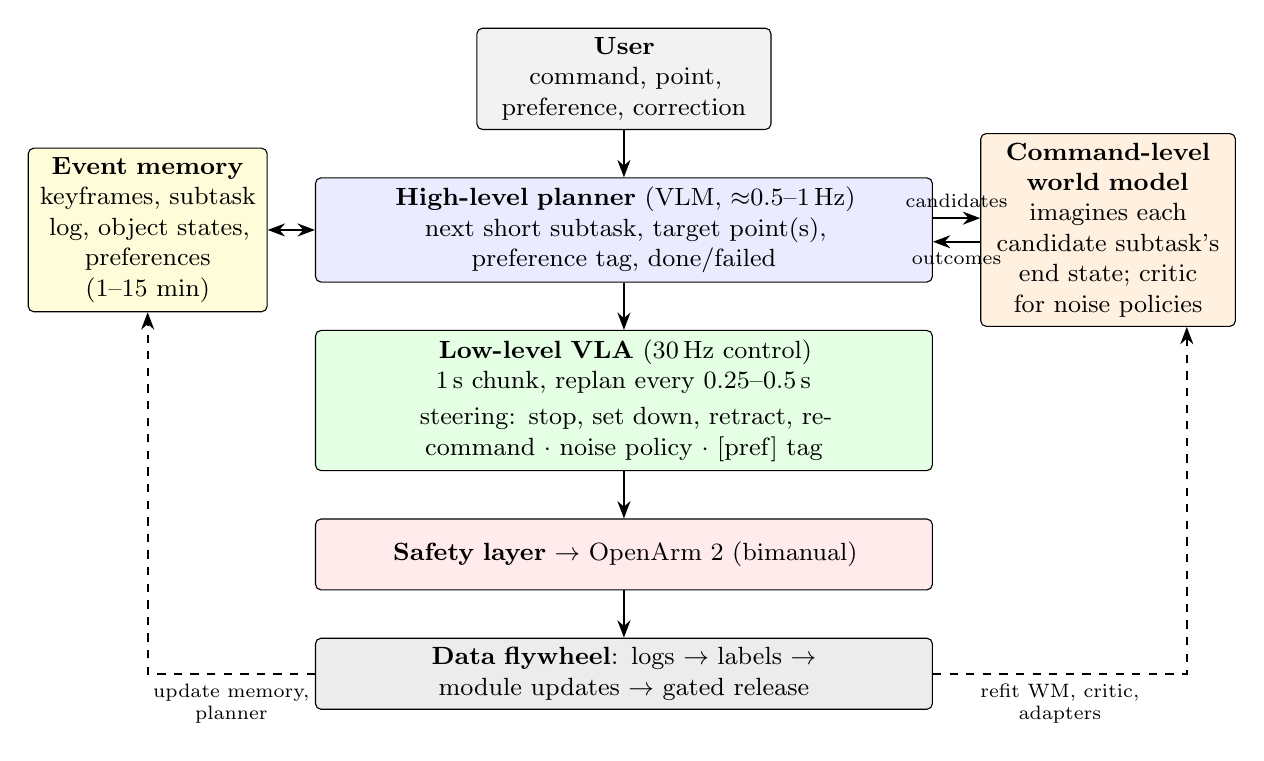
\begin{tikzpicture}[font=\small, node distance=6mm and 6mm,
  box/.style={draw, rounded corners=2pt, align=center, minimum height=9mm, text width=3.5cm, fill=#1},
  box/.default=white, arr/.style={-{Stealth[length=2.2mm]}, thick}]
\node[box=gray!10] (user) {\textbf{User}\\command, point, preference, correction};
\node[box=blue!8, below=of user, text width=7.6cm] (plan) {\textbf{High-level planner} (VLM, $\approx$0.5--1\,Hz)\\next short subtask, target point(s), preference tag, done/failed};
\node[box=yellow!15, left=of plan, text width=2.8cm] (mem) {\textbf{Event memory}\\keyframes, subtask log, object states, preferences (1--15 min)};
\node[box=green!10, below=of plan, text width=7.6cm] (vla) {\textbf{Low-level VLA} (30\,Hz control)\\1\,s chunk, replan every 0.25--0.5\,s\\[2pt] steering: stop, set down, retract, re-command $\cdot$ noise policy $\cdot$ [pref] tag};
\node[box=orange!12, right=of plan, text width=3.0cm] (wm) {\textbf{Command-level world model}\\imagines each candidate subtask's end state; critic for noise policies};
\node[box=red!8, below=of vla, text width=7.6cm] (safe) {\textbf{Safety layer} $\rightarrow$ OpenArm~2 (bimanual)};
\node[box=gray!15, below=of safe, text width=7.6cm] (fly) {\textbf{Data flywheel}: logs $\rightarrow$ labels $\rightarrow$ module updates $\rightarrow$ gated release};
\draw[arr] (user) -- (plan);
\draw[arr] (plan) -- (vla);
\draw[{Stealth[length=2.2mm]}-{Stealth[length=2.2mm]}, thick] (mem) -- (plan);
\draw[arr] ([yshift=1.5mm]plan.east) -- node[above, font=\scriptsize]{candidates} ([yshift=1.5mm]wm.west);
\draw[arr] ([yshift=-1.5mm]wm.west) -- node[below, font=\scriptsize]{outcomes} ([yshift=-1.5mm]plan.east);
\draw[arr] (vla) -- (safe);
\draw[arr] (safe) -- (fly);
\draw[arr, dashed] (fly.west) -| node[pos=0.25, below, font=\scriptsize, align=center]{update memory,\\planner} (mem.south);
\draw[arr, dashed] (fly.east) -| node[pos=0.25, below, font=\scriptsize, align=center]{refit WM, critic,\\adapters} ([xshift=10mm]wm.south);
\end{tikzpicture}
\caption{End-to-end stack. Long-horizon reasoning lives in the planner and memory; the VLA only executes short subtasks; steering modules leave the VLA weights unchanged by default.}
\end{figure}

\begin{small}
\begin{longtable}{@{}P{2.4cm}P{4.3cm}P{4.6cm}P{3.6cm}@{}}
\toprule
\textbf{Component} & \textbf{Role / interface} & \textbf{Evidence (this report)} & \textbf{Candidates} \\
\midrule\endhead
Planner & task + images + memory $\rightarrow$ subtask text, target points, tags, done & Nudge from target points +16--26 pts; missions 5/24 with vs 0/24 without & Qwen3-VL-4B fine-tuned (Apache-2.0) \\
Event memory & logs events, re-issues task, tracks counts & +46 pts (instruction loss); 3$\times$ on repetition tasks & own module \\
Low-level VLA & executes 2--10\,s subtasks in 1\,s chunks & short subtasks are what VLAs do well & LingBot-VLA 2.0, GR00T N1.7 (OpenArm ckpt), \pzf \\
Steering adapters & nudge (target), noise policy (no target), CFG/[pref] & Table~\ref{tab:steer}; PrefPI \S\ref{sec:res-pref} & per-skill, refreshed in the flywheel \\
World model + critic & imagines candidate subtasks' outcomes (picture goals); critic trains noise policies & 26/80 vs 3/80 missions, 53/53 picture goals; gradient planning 4$\times$ faster & own small model on robot data; FLUX~3 Action (research) \\
Safety & limits, collision, e-stop, takeover & -- & -- \\
\bottomrule
\end{longtable}
\end{small}

\subsection{Data preprocessing pipeline}
\begin{enumerate}
\item \textbf{Standardise} to LeRobot v3: fixed control rate, synchronised timestamps, consistent camera names and orientation, joint angles in rad, fixed arm order, gripper 0--1 with one convention; automatic checks for gripper sign and image orientation (both bit us, \S\ref{sec:dataq}).
\item \textbf{Clean}: drop/flag frame drops, desync, truncation; trim idle segments; per-embodiment normalisation statistics frozen per release.
\item \textbf{Annotate}: subtask segmentation (VLM proposals, human verification); events from gripper/force signals (grasp, release, contact); target points (gripper position at grasp projected into images); success and progress labels; metadata (speed, smoothness, operator, mistakes, recoveries).
\item \textbf{Split} by scene, object, day and operator; hold out whole tasks.
\item \textbf{Derive} per-module sets: VLA (subtask text, optional target/tag, condition dropout for CFG), planner (images + history $\rightarrow$ next subtask/point/done), world model (observation, chunk $\rightarrow$ future latents), critic (state $\rightarrow$ progress/success), memory (event timelines).
\end{enumerate}

\subsection{Post-training and continuous improvement}
\begin{small}
\begin{tabularx}{\textwidth}{lYY}
\toprule
Layer & Method & Lesson from our runs \\
\midrule
Steering policies (first, cheapest) & Dyna loop: on-policy data $\rightarrow$ refit world model + critic $\rightarrow$ backpropagate into the noise policy; or success-filtered noise BC & Reversible; do not transfer to unseen situations, so refresh per skill \\
VLA (rarer, gated) & filtered BC / DAgger on takeovers; PrefPI for style; value-conditioned (good/bad tag from the critic) training & \textbf{Anchor with original demonstrations} ($\approx$50\%), LoRA, small LR: one round on own rollouts made G0.5 11\% slower \\
Planner & SFT on corrected plans; RL on verified success & planner errors are a main mission failure mode \\
World model, critic & continual refit on all logs & on-policy data keeps the model accurate where the policy goes \\
\bottomrule
\end{tabularx}
\end{small}
\medskip\noindent Release gates: held-out offline set + imagined rollouts; simulator regression suite; small paired real-robot A/B on shared start states (McNemar); versioned release with rollback.

%==================================================================
\section{Data quality assessment}
\label{sec:dataq}
\begin{small}
\begin{longtable}{@{}P{2.7cm}P{5.6cm}P{3.8cm}P{3.2cm}@{}}
\toprule
\textbf{Dataset} & \textbf{Issues found} & \textbf{Impact} & \textbf{Fix / status} \\
\midrule\endhead
LIBERO (LaWAM merged set, 1,693 demos, 273k frames) & Gripper action sign inverted relative to G0.5's data & Frozen G0.5 loss 2.44 vs 0.072; a first adapter silently learned to undo the sign & Converted copy ($a_6\rightarrow1-a_6$); run discarded \\
& AV1 video requiring specific FFmpeg/torchcodec builds & Training/decoding failures & Pinned decoder build \\
& Normalisation must be the released checkpoint's & Mismatched stats shift actions & Released stats enforced \\
RoboCasa365 (50 target tasks, 97\,GB) & Inconsistent subtask feature columns across task datasets; per-model action conventions (12-D, engine order, gripper $\pm$1) & Aggregation failed; wrong action order would score 0\% & Columns dropped; adapters checked against dataset layout \\
DROID household subset & Keyword-based task categories (noisy); 320$\times$180 at 15\,Hz (downsampled); many clips shorter than model windows; in-distribution for every evaluated world model & Optimistic, low-resolution evaluation; category labels imperfect & Report as in-distribution; OpenArm data needed \\
PrimeBot (washer tasks, X2W robot) & Partially downloaded, not assessed & -- & paused \\
Self-generated rollouts (steering, PrefPI) & Inversion error for recorded noises (73/1,200 records $>$0.1); success-only recording; distribution shift from the steering condition & Noisy labels; drift when retraining on own data & Error filter; anchoring with demos (testing) \\
OpenArm 2 collected data & Not yet on the cluster & Blocks real-robot claims & Run the checks of \S\ref{sec:pipeline} on ingest \\
\bottomrule
\end{longtable}
\end{small}
\noindent\textbf{Checks to run on the OpenArm data at ingest}: per-episode completeness and timing (frame drops, camera/joint sync jitter); calibration drift between days; gripper and joint conventions per arm; image orientation and exposure; action/state ranges vs hardware limits; idle fraction; label coverage (subtasks, success, events); operator and scene balance; duplicates; held-out split integrity.

%==================================================================
\section{Gaps and limitations}
\label{sec:gaps}
\begin{enumerate}
\item \textbf{No real-robot evidence.} Every result is simulation (LIBERO, RoboCasa365) or offline on public recordings. The OpenArm data cannot be accessed for now, so real-robot claims (C1, C4, C8--C10) stay open; the closest available proxies are DROID's real household recordings (offline) and bimanual simulation (RoboTwin~2.0, which LingBot-VLA~2.0 supports natively).
\item \textbf{Benchmark ceiling and synthetic probes.} LIBERO is at 98.9\%; the command-switch probe is synthetic; 100 trials per cell, 2 trials per RoboCasa task, 2--4 seeds for planning.
\item \textbf{World-model evaluation is in-distribution and low resolution.} DROID is in all evaluated models' training data; Cosmos~3 was only tested in its Edge size (Nano does not fit our GPUs).
\item \textbf{Low-level policy comparison is incomplete.} GR00T severely under-trained; \pzf\ disadvantaged by the shared replanning interval; LingBot-VLA 2.0 and G0.5 not yet on RoboCasa365; no OpenArm bake-off.
\item \textbf{Steering generalisation and the improvement loop.} Learned noise policies do not transfer to unseen command pairs; the model-based gain is modest and over-predicted by the learned model, and a second improvement round lost it again.
\item \textbf{Preference drift.} PrefPI's self-training drifts the policy and collapses success after 5 rounds; the anchoring fix is untested.
\item \textbf{Memory tests do not reflect real-life memory needs.} The main memory probe withdraws the instruction after 2\,s and asks the memory to re-issue it, which a deployed system would never need: it keeps its command. The repetition tasks gain mainly with an oracle counter. Real household memory needs are untested: resuming a plan after an interruption without redoing finished steps, state that is no longer visible (items inside a closed drawer or a washer drum), progress counts on repetitive tasks, and standing instructions given minutes earlier. All memory results are on $\le$1\,min episodes.
\item \textbf{Planner robustness and privileged targets.} The zero-shot planner mis-parses some requests and perceives simulated scenes poorly. In the mission benchmark the nudge's target point comes from a fixed per-task table rather than from the planner, which favours the nudge over the target-free noise policies; on hardware the point must come from the planner or a person (C1).
\item \textbf{Licences.} The best-performing research components (G0.5, Awomo, FLUX~3 Action, RoboJEPA) are restricted; FLUX's licence forbids distilling its outputs into our models.
\item \textbf{Compute.} Only T4/V100 are available at scale; H200 access is queued; several published recipes (GR00T, LingBot, FLUX fine-tuning) are infeasible on the available GPUs. When another user's week-long job held every T4, the G0.5 experiments moved to V100s (a Volta build of the environment; G0.5's linear-attention prefill on its fp32 PyTorch path because the Triton kernel does not compile on Volta); the same held-out episodes give the same outcome on T4 and V100 in 89--93\% of cases (nudge 39 vs 42/100, switch 13 vs 8/100), and every comparison in this report pairs conditions run on the same hardware.
\end{enumerate}

%==================================================================
\section{Claims we need to verify}
\label{sec:claims}
\begin{small}
\begin{longtable}{@{}P{0.5cm}P{4.3cm}P{3.3cm}P{4.3cm}P{2.4cm}@{}}
\toprule
\# & \textbf{Claim} & \textbf{Current evidence} & \textbf{Test and success criterion} & \textbf{Where} \\
\midrule\endhead
C1 & After a change of mind, stopping, retracting and re-commanding makes the robot follow the new command & sim missions: 51/53 vs 7/55 without steering and 26/53 with a nudge; VLM-pointed nudge = perfect target & Real change-of-mind probe, 10 tasks $\times$ 10 states: retract vs nudge (VLM point) vs none; safe retraction while holding objects & OpenArm \\
C2 & A learned noise policy steers without a target for trained skills & sim: 45\% vs 29\%; no transfer & Real, per skill; $\geq$ nudge on trained skills & OpenArm \\
C3 & Planner + short low-level horizons raise multi-step success & sim missions: 5/24 vs 0/24 without planner ($p=0.06$); planner wrong in 2/8 missions & Remaining E2E arms; 3 seeds; fine-tuned planner; RoboCasa composite with planner $>$ plain (paired) & sim $\rightarrow$ OpenArm \\
C4 & External event memory is needed for real household memory demands & sim: resume after interruption 23--27/40 with an activity log vs 0--7/40 without; rule memory 0/30 vs 20/30 instruction violations; hidden repetition count in closed loop: activity-log 20.8\% and video memory 19.2\% vs 4--6\% Markovian ($p\le0.003$) & Interrupt-and-resume, out-of-view state, progress counts and standing instructions, with event memory vs current-view-only vs full-transcript planners; then OpenArm washer loading (occluded count) and interrupted folding & OpenArm \\
C5 & A world model improves the full system & sim, realistic inputs: command-level model reads 53/53 picture goals, missions 26/80 vs 3/80 ($p=1.6\times10^{-6}$); as a motion verifier no gain (also with diverse proposals); 1.6\,s goal reading at chance & Supported at the subtask level (sim, closed 10-command set); test open-vocabulary commands, a fine-tuned planner as a stronger control, and OpenArm & sim $\rightarrow$ OpenArm \\
C6 & Anchored PrefPI changes style without drift or collapse & sim: height +25\% net of drift (both variants), anchoring removes $\sim$3\,cm drift; speed preference not learned; success 85\% at round 5 & Anchored chains: preference metric up, success $\geq$90\%, other metrics within noise & sim $\rightarrow$ OpenArm \\
C7 & The improvement loop is monotonic across rounds & round 1 +6/+9; round 2 --6/--9 (overconfident critic); round 2 with early-stopped critic = round 1; round 3 with fresh start states = round 2 (75 vs 80/200); applied to the VLA's weights: collapse (0/200) or no effect & Not supported beyond round 1 in noise space; never into the weights. Next: human corrections or real successes as the new data source, critic ensembles; then OpenArm & sim $\rightarrow$ OpenArm \\
C8 & A commercially usable VLA meets the target success on OpenArm tasks & none on OpenArm & Bake-off: LingBot-VLA 2.0, GR00T N1.7, \pzf, equal budget; pick by success and latency & OpenArm \\
C9 & World-model rankings hold out of distribution & DROID in-distribution only & Evaluate on OpenArm recordings & offline \\
C10 & The full stack meets real-time latency on robot hardware & component timings only & End-to-end latency $<$ control budget on the robot GPU & OpenArm \\
\bottomrule
\end{longtable}
\end{small}

%==================================================================
\section{Compute}
\label{sec:compute}

\subsection{Measured costs on the current cluster}
\begin{small}
\begin{tabularx}{\textwidth}{Ylr}
\toprule
Workload & Hardware & Measured time\meas \\
\midrule
LIBERO steering evaluation, 100 episodes & 1$\times$T4 & 15--17\,min \\
Noise-policy data recording, per job & 1$\times$T4 & 16--40\,min \\
SuperMimic-style policy improvement (backprop through G0.5's sampler) & 1$\times$T4 & 5.6\,s per iteration \\
PrefPI training round, 3,000 / 1,500 steps (effective batch 12, 2.7\,s/step) & 1$\times$T4 & 2.4 / 1.2\,h \\
PrefPI rollouts, 40 episodes & 1$\times$T4 & 8--12\,min \\
End-to-end missions (planner + memory + WM + G0.5), ablation arm of 24 missions & 2$\times$T4 & 12--14\,min per arm \\
RoboCasa365, 100 episodes, \pzf\ / GR00T & 4$\times$T4 & 2.4\,h / 1.2\,h per job \\
RoboCasa365, Awomo fp16 & V100 & 0.25\,s per control step \\
GR00T N1.7 fine-tune, 6k steps, batch 16, 8-bit AdamW & 1$\times$V100 & 1.6\,h \\
FLUX 3 Action, 72 prediction windows (bf16, partial CPU offload) & 3$\times$T4 & 0.9\,h each (119\,s/window) \\
FLUX 3 Action, 72 windows $\times$ 3 variants (native bf16) & 1$\times$A100 & 2--4\,s/window; 15\,min for all three \\
Cosmos 3 Edge-Policy, 72 windows & 3$\times$T4 & $\approx$2\,min/window \\
RoboJEPA 1B evaluation, 96 clips & 1$\times$T4 & 79\,min \\
RoboJEPA planning, 2 episodes: CEM / gradient & 1$\times$T4 & 38 / 9.4\,min \\
\bottomrule
\end{tabularx}
\end{small}

\subsection{Projected budget for the full end-to-end programme}
\begin{small}
\begin{tabularx}{\textwidth}{Yrr}
\toprule
Workstream & Simulation / offline & Real robot \\
\midrule
E2E mission benchmark: 6 arms $\times$ 24 missions, then $\times$3 seeds and more missions & $\le$100, then $\le$300 T4-h\est & -- \\
RoboCasa planner study (composite, 2 sets $\times$ 2 trials, 3 seeds) & $\approx$60 T4-h\est & -- \\
Steering + improvement loop, 3 rounds (record, refit, improve, evaluate) & $\approx$40 T4-h\est & 3 rounds $\times\approx$200 trials \\
PrefPI anchored, 2 objectives $\times$ 8 rounds (T4) & $\approx$30 T4-h\est & $\approx$150 labelled episodes per objective \\
Low-level bake-off on OpenArm data: LingBot-VLA 2.0 (6B), GR00T N1.7 (3B), \pzf\ (3B), equal budget & 600--1,500 H200-h\est & 3 policies $\times$ 10 tasks $\times$ 20 trials \\
Own world model + critic on OpenArm data & 100--200 H200-h\est & -- \\
Planner fine-tune (Qwen3-VL-4B, LoRA) on subtask annotations & 50--100 H200-h\est & -- \\
FLUX 3 Action fine-tune on folding (research arm) & 200--400 H200-h\est & 2 tasks $\times$ 20 trials \\
\midrule
\textbf{Total} & \textbf{$\approx$430 T4-h + 1,000--2,200 H200-h}\est & \textbf{$\approx$2--3 robot-weeks}\est \\
\bottomrule
\end{tabularx}
\end{small}
\noindent The E2E figure is an upper bound: the first two arms ran for hours, while the ablation arms finished 24 missions in 12--14\,min; the difference is not yet profiled. The T4 part fits the current allowance (10 T4 per user) in about 2 days of continuous use. The H200 part needs 250--550 hours of continuous use at the current allowance of 4 H200 per user (1.5--3.5 weeks), and longer in practice because the H200 partition is fully booked. A dedicated 8$\times$H200 node would finish it in 5--12 days. \textbf{On-robot inference}: one RTX~4090/5090-class GPU (LingBot-VLA 2.0 $\approx$130\,ms per chunk on a 4090D; Qwen3-VL-4B at $\approx$1\,Hz; a small world model scoring 4--8 chunks per replan); FLUX~3 Action needs Ada/Hopper-class GPUs for its FP8 packages.

%==================================================================
\clearpage
\section{Current status on the cluster and next steps}
\label{sec:status}
\begin{small}
\begin{xltabular}{\textwidth}{>{\raggedright\arraybackslash}p{3.1cm}YY}
\toprule
Workstream & What is being tested & State \\
\midrule
\endhead
E2E missions & all 6 arms (Table~\ref{tab:e2e}) & finished \\
Fair steering comparison & change-of-mind step, 80 missions per arm: nudge with the table target (privileged), a simulated human click (4\,px noise, lifted with depth), the planner's own point (lifted with depth); DSBC v2; model-based round 1; no steering & finished: retract-and-re-command best (\S\ref{sec:res-e2e}) \\
Memory, level 1 (realistic needs) & interrupt-and-resume and standing-instruction missions in the kitchen with the full stack; planner with an event memory (plan, own activity log, camera checks; no simulator signals) vs the whole conversation transcript vs current view only; 70 episodes per arm; with RoboBrain 2.5 and with Qwen3-VL-4B as the planner & finished, plus a rule-memory arm (\S5.3) \\
Memory, level 2 (state the frame cannot show) & LIBERO-Mem swap/rotate of identical bowls and cheese-to-basket tasks; G0.5 fine-tuned on step episodes; next-step instructions from a video-memory decoder vs a current-frame decoder vs the original instruction vs an oracle; 20 held-out starts per task & finished; results in \S5.3 \\
Planner on RoboCasa365 & \pzf\ with Qwen3-VL-4B subtasks, composite seen/unseen & finished: no gain (\S\ref{sec:res-e2e}); next: constrain sub-goals to \pzf's skill vocabulary \\
Improvement loop & SuperMimic-style steering rounds 2 and 3 (fresh start states); the same objective training G0.5's own action expert & finished: rounds plateau at the nudge's level; weight training collapses (0/200) or, tightly anchored, does nothing (\S\ref{sec:res-steer}) \\
World model in missions & motion verifier with diverse proposals vs random pick; goal reading by 1.6\,s imagination; command-level end-state model vs the planner & finished: only the command-level model helps, 26/80 vs 3/80 missions (Table~\ref{tab:wm-missions}) \\
Weak-skill noise policy & LIBERO-Mem bowl moves and baskets: noise policy trained on step-level successes vs G0.5's own noise vs zero noise, oracle and memory-decoder step instructions, 20 held-out starts per task & finished: the learned noise policy hurts (9 vs 27/80); zero noise helps (36 vs 27/80, baskets 35 vs 26/40); bowl moves stay weak (\S5.3) \\
Preferences & anchored PrefPI (speed, height, 50\% demonstrations); original chains & finished (5 anchored rounds; 8 original rounds) \\
World-action models & FLUX~3 Action base and distilled in native bf16 & finished on an A100: step-distilled best (0.77$\times$ hold-still overall), base reproduces the T4 port \\
Low-level bake-off & LingBot-VLA 2.0 (6B) post-training on RoboCasa365, then the shared-harness evaluation against \pzf, GR00T and Awomo & running on one A100 since 25 October (bf16 weights, AnyPrecisionAdamW, bf16 autocast; 1.17\,s/step, 200k steps, $\approx$65\,h); the step-5k checkpoint passes the harness end to end (1/50, expected this early); step-50k check queued \\
Retraction as teacher & partial retractions (0--100\% of the path) after a mid-task change of mind; a vision student (both cameras, state, commands) learns the shortest back-off that keeps success; held-out test vs full retraction and release only & running (first results: release only 2/41, full retraction 35/41) \\
\bottomrule
\end{xltabular}
\end{small}
\textbf{Next}: ingest OpenArm data through the preprocessing pipeline; run the low-level bake-off (C8); repeat C1--C4 on hardware; train our own world model on OpenArm data; then the full flywheel with gated releases.

%==================================================================
\begin{thebibliography}{99}\small
\bibitem{pi0} K.~Black et al. \pz: A vision-language-action flow model for general robot control. RSS, 2025.
\bibitem{pi05} K.~Black et al. \pzf: a vision-language-action model with open-world generalization. CoRL (PMLR 305), 2025.
\bibitem{pi07} Physical Intelligence. \pzs. arXiv:2604.15483, 2026.
\bibitem{g05} Galaxea. G0.5. arXiv:2608.11739, 2026. \url{https://github.com/OpenGalaxea/GalaxeaVLA}
\bibitem{gr00t} NVIDIA. Isaac GR00T N1.7. \url{https://github.com/NVIDIA/Isaac-GR00T}
\bibitem{lingbot2} Robbyant. LingBot-VLA 2.0. 2026. \url{https://github.com/robbyant/lingbot-vla-v2}
\bibitem{awomo} Awomo-0.5. \url{https://github.com/Awomo-WestlakeDI/Awomo-0.5}
\bibitem{vla_forget} Pretrained vision-language-action models are surprisingly resistant to forgetting in continual learning. arXiv:2603.03818, 2026.
\bibitem{robojepa} RoboJEPA: Scaling robotic latent world models. arXiv:2610.10515, 2026.
\bibitem{lawam} LaWAM. arXiv:2606.15768, 2026.
\bibitem{flare} FLARE: Robot learning with implicit world modeling. arXiv:2505.15659, 2025.
\bibitem{cosmos3} NVIDIA. Cosmos 3. \url{https://huggingface.co/collections/nvidia/cosmos3}
\bibitem{flux3a} Black Forest Labs. FLUX 3 Action. \url{https://huggingface.co/black-forest-labs/flux-3-action-droid}
\bibitem{openwam} OpenWAM: An open, modular exploration towards systematic world-action model pretraining. arXiv:2609.07398, 2026.
\bibitem{dreamerv3} D.~Hafner et al. Mastering diverse domains through world models (DreamerV3). 2023.
\bibitem{tdmpc2} N.~Hansen et al. TD-MPC2: Scalable, robust world models for continuous control. ICLR, 2024.
\bibitem{shac} J.~Xu et al. Accelerated policy learning with parallel differentiable simulation (SHAC). ICLR, 2022.
\bibitem{supermimic} Q.~Liao, Y.~Shao, J.~Long, K.~Zakka, R.~Horowitz, P.~Abbeel, K.~Sreenath. SuperMimic: Scaling humanoid whole-body control with one differentiable world model. CoRL, 2026. arXiv:2610.28480.
\bibitem{cfg} J.~Ho, T.~Salimans. Classifier-free diffusion guidance. arXiv:2207.12598, 2022.
\bibitem{cfgrl} K.~Frans, S.~Park, P.~Abbeel, S.~Levine. Diffusion guidance is a controllable policy improvement operator. arXiv:2505.23458, 2025.
\bibitem{frs} Improving robotic generalist policies via flow reversal steering. arXiv:2606.13675, 2026.
\bibitem{dsrl} A.~Wagenmaker et al. Steering your diffusion policy with latent space reinforcement learning. CoRL, 2025.
\bibitem{flowdagger} FlowDAgger: Human-in-the-loop adaptation of generative robot policies in latent space. arXiv:2607.08877, 2026.
\bibitem{vls} VLS: Steering pretrained robot policies via vision-language models. arXiv:2602.03973, 2026.
\bibitem{imagrecovery} Imagining recovery: Inference-time counterfactual realignment for vision-language-action models. arXiv:2608.14822, 2026.
\bibitem{prefpi} S.~Rho, W.~Kim, D.~Xu, S.~Ha. PrefPI: Preference-guided steering into out-of-distribution behaviors. arXiv:2609.40165, 2026.
\bibitem{diffdpo} B.~Wallace et al. Diffusion model alignment using direct preference optimization. CVPR, 2024.
\bibitem{fdpp} Y.~Chen et al. FDPP: Fine-tune diffusion policy with human preference. ICRA, 2025.
\bibitem{dppo} A.~Z.~Ren et al. Diffusion policy policy optimization. ICLR, 2025.
\bibitem{flowpro} Y.~Wu et al. FlowPRO: Reward-free reinforced fine-tuning of flow-matching VLAs via proximalized preference optimization. arXiv:2606.05468, 2026.
\bibitem{liberomem} Chung et al. LIBERO-Mem. arXiv:2511.11478, 2025.
\bibitem{mikasa} MIKASA-Robo-VLA: Benchmarking memory in VLA models for long-horizon manipulation. arXiv:2610.00604, 2026.
\bibitem{3dmem} 3D-Mem: 3D scene memory for embodied exploration and reasoning. CVPR, 2025. arXiv:2411.17735.
\bibitem{robobrain} BAAI. RoboBrain 2.0 technical report. arXiv:2507.02029, 2025.
\bibitem{qwen3vl} Qwen Team. Qwen3-VL. 2025.
\bibitem{libero} B.~Liu et al. LIBERO: Benchmarking knowledge transfer for lifelong robot learning. NeurIPS, 2023.
\bibitem{liberopro} LIBERO-PRO: Towards robust and fair evaluation of VLA models beyond memorization. arXiv:2510.03827, 2025.
\bibitem{robocasa365} RoboCasa365: A large-scale simulation framework for training and benchmarking generalist robots. arXiv:2603.04356, 2026.
\bibitem{droid} A.~Khazatsky et al. DROID: A large-scale in-the-wild robot manipulation dataset. RSS, 2024.
\bibitem{agibot} Scaling bimanual household manipulation from 1,500 hours of demonstrations to on-policy corrections. arXiv:2609.03591, 2026.
\end{thebibliography}

\end{document}
